\section{Arquitectura del Sistema}

La arquitectura del sistema se basa por completo en el uso de \textit{Next.js}, un framework de \textit{React} que permite la creación de aplicaciones web, con la funcionalidad clave de un backend integrado. Desde la versión 13 de \textit{Next.js} se introdujo el concepto de \textbf{App Router}, que crea las rutas de la web en base a la organización de las carpetas dentro del proyecto. Junto a esto, se introdujeron los \textbf{Route Handlers}, que permiten la creación de endpoints API REST de la misma manera, creando un backend integrado que hace de intermediario entre el cliente y los servicios externos. De esta manera, se consigue una arquitectura notablemente más simplificada, además de segura, ya que se puede controlar la exposición de datos sensibles al cliente.

Otra caracterísitica muy útil de \textit{Next.js}, son los \textbf{Server Components}, que permiten renderizar componentes en el servidor en lugar del cliente. Solo aquellos componentes que sean necesarios serán enviados y ejecutados en el cliente, mejorando el rendimiento y la seguridad. Estos componentes pueden realizar llamadas a los endpoints proporcionados por los \textit{Route Handlers}, recreando los roles de un sistema cliente-servidor tradicional. En el diagrama \ref{fig:arquitectura_sistema} se pueden ver representadas estas interacciones.

\begin{figure}[H]
    \centering
    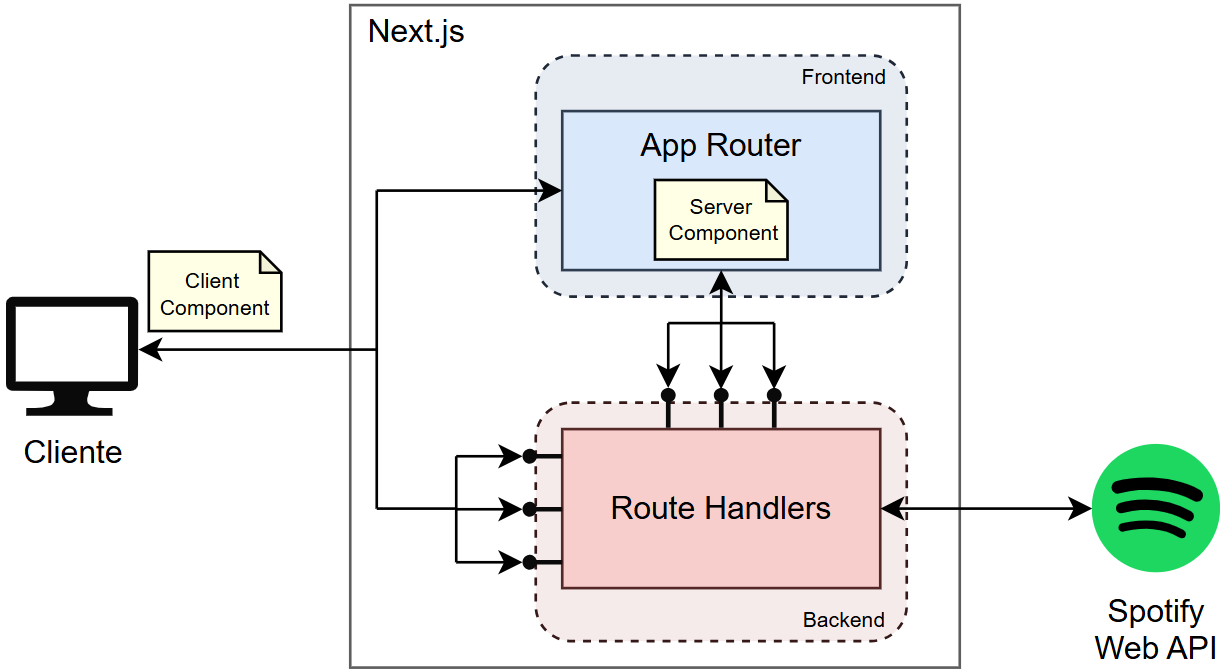
\includegraphics[width=0.85\textwidth]{figures/arquitectura_sistema.png}
    \caption{Diagrama de la arquitectura del sistema haciendo uso de \textit{Next.js}.}
    \label{fig:arquitectura_sistema}
\end{figure}

% TODO: Igual quitar esta subsection y que los subsubsection sean directamente en el apartado de arquitectura
\subsection{Estructura de Rutas y Endpoints en Next.js}

Como se ha mencionado anteriormente, la estructura de rutas y endpoints en \textit{Next.js} se basa en la organización de las carpetas y archivos dentro del proyecto. En los siguientes apartados se describirán cuáles son y cómo se organizan en este desarrollo.

\subsubsection{Rutas del Frontend}

Usando el \textit{App Router}, las rutas del frontend se organizan en la carpeta \texttt{app/}, donde cada subcarpeta representa una ruta específica en la web. Dentro de cada carpeta se pueden encontrar archivos específicos que siguen una convención de nombres, y que definen su función. Las más importantes son:

\begin{itemize}
    \item \texttt{layout.tsx}: Define el diseño compartido de los componentes que se encuentran anidados en las subcarpetas interiores.
    \item \texttt{page.tsx}: Contiene el contenido principal de una ruta específica. Representa la página renderizada cuando el usuario accede a esa ruta. \textbf{Para que una página sea accesible, debe existir un archivo \texttt{page.tsx} en la carpeta correspondiente}.
    \item \texttt{loading.tsx}: Muestra un indicador de carga mientras se obtienen datos o se renderizan componentes en una página.
    \item \texttt{error.tsx}: Gestiona errores específicos de una página, mostrando mensajes o interfaces para el usuario en caso de fallos.
\end{itemize}

En el caso de este proyecto, la jerarquía de carpetas que genera las páginas routeables de la web es la siguiente:

\begin{verbatim}
    app/
    ├── home/
    │   └── page.tsx (Ruta: /home)
    ├── stats/
    │   └── page.tsx (Ruta: /stats)
    └── page.tsx (Ruta: /)
\end{verbatim}

La ruta \texttt{/} (raíz) es la página principal, en donde el usuario puede iniciar sesión. Las rutas \texttt{/home} y \texttt{/stats} representan las páginas de estadísticas básicas y estadísticas avanzadas, respectivamente. En cada caso, el archivo \texttt{page.tsx} define el contenido principal de la página y es posible añadir otros archivos como \texttt{layout.tsx}, \texttt{loading.tsx} o \texttt{error.tsx} para mejorar la experiencia del usuario.

\subsubsection{Endpoints del Backend}

En el caso de la creación de endpoints mediante los \textit{Route Handlers}, la estructura de carpetas es similar a la de las rutas del frontend, pero con la diferencia de que cada subcarpeta dentro de \texttt{app/api/} contiene un archivo \texttt{route.ts} que define el comportamiento del endpoint asociado. \textbf{Para que un endpoint sea accesible, debe existir un archivo \texttt{route.ts} en la carpeta correspondiente}.

La estructura de carpetas para los endpoints de este proyecto es la siguiente:

\begin{verbatim}
    app/
    └── api/
        ├── auth/
        │   ├── callback/route.ts
        │   ├── login/route.ts
        │   └── logout/route.ts
        ├── home/
        │   ├── recently-played/route.ts
        │   ├── top-artists/route.ts
        │   ├── top-genres/route.ts
        │   ├── top-tracks/route.ts
        │   └── user-profile/route.ts
        └── stats/
            ├── estaciones-musicales/route.ts
            ├── hall-of-fame/route.ts
            ├── huella-del-dia/route.ts
            ├── indice-de-resonancia/route.ts
            ├── la-bitacora/route.ts
            └── tus-decadas/route.ts
\end{verbatim}

Los endpoints en \texttt{/api/auth/} gestionan el incio de sesión del usuario, mientras que los de \texttt{/api/home/} y \texttt{/api/stats/} se encargan de obtener y procesar los datos necesarios para las estadísiticas. El contenido del fichero \texttt{route.ts} sigue una convención concreta que \textit{Next.js} reconoce y utiliza para gestionar las peticiones, la cual se explicará con más detalle en el capítulo de \nameref{ch:implementacion}.

\section{Diagrama de Componentes de React}

Los componentes en \textit{React} son las piezas fundamentales para construir interfaces de usuario. Cada componente puede ser reutilizable, contener su propio estado y lógica, y ser combinado con otros para formar estructuras más complejas. Además, en \textit{React}, las interfaces se suelen diseñar en forma de jerarquías de componentes, en las que los componentes ``padre'' organizan y controlan el comportamiento y la presentación de los componentes ``hijo''. Esta organización jerárquica facilita el mantenimiento y la escalabilidad del código, ya que cada componente tiene una responsabilidad definida.

En este proyecto, se ha creado una jerarquía de componentes (diagrama \ref{fig:componentes_react}) que refleja las diferentes funcionalidades de la aplicación. A la hora de construir la web, \textit{Next.js} se encarga de anidar los componentes necesarios y renderizarlos, o enviarlos al cliente, según sea necesario.

\begin{figure}[H]
    \centering
    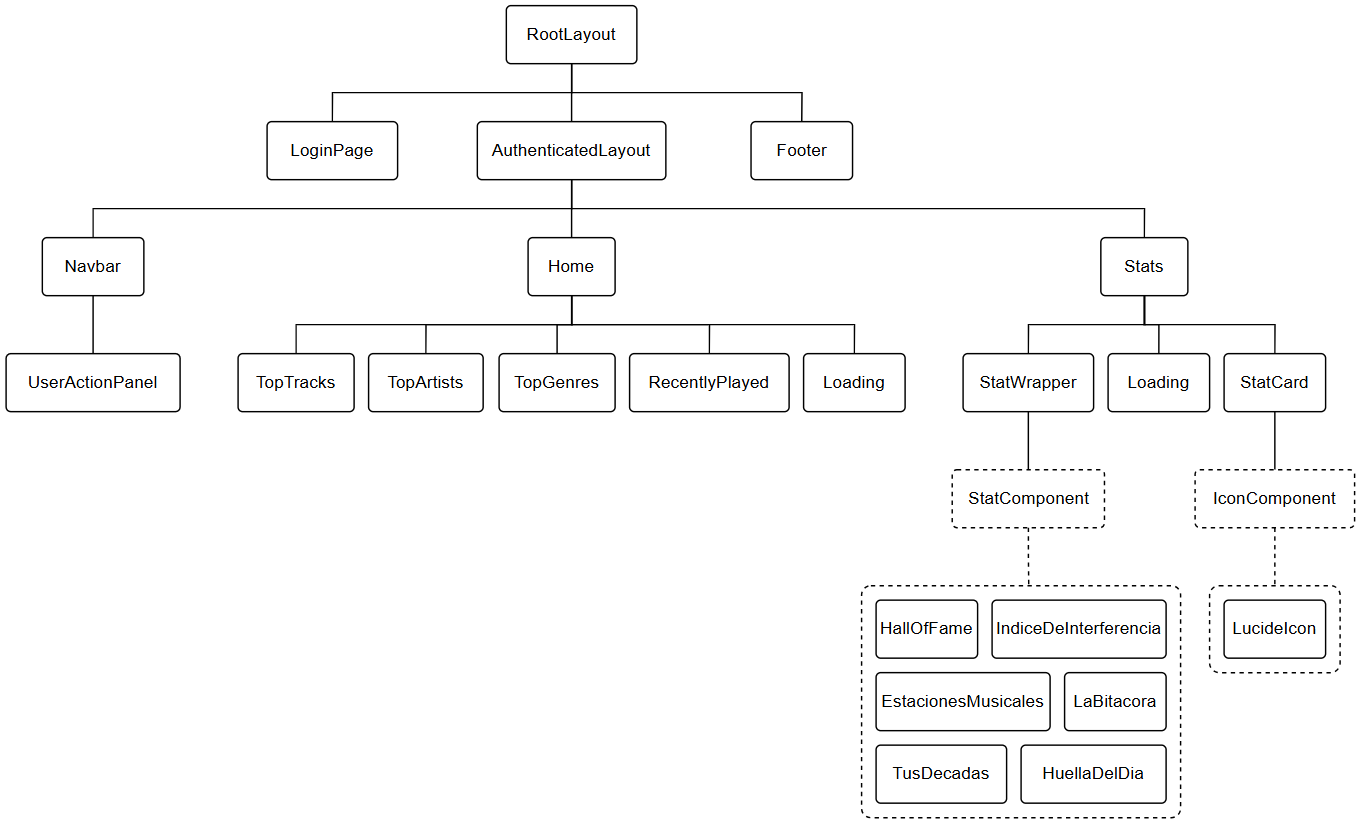
\includegraphics[width=0.9\textwidth]{figures/componentes_react.png}
    \caption{Diagrama de la jerarquía de componentes de React creados en el proyecto.}
    \label{fig:componentes_react}
\end{figure}

La mayoría de los componentes están definidos de manera explícita y son renderizados cuando se llegue a una ruta en concreto, pero hay otros componentes que se cargan dinámicamente, es decir, el contenido que aparece en su lugar puede variar en función de las acciones del usuario o del contexto del componente. Se podría considerar que el componente hijo temporal, se ``transforma'' en otro componente que toma su lugar. En este proyecto, se han definido dos componentes que se comportan así:

\begin{itemize}
    \item \textbf{StatComponent}: Se utiliza para mostrar una de las seis estadísticas disponibles, cada una siendo un componente autocontenido. Dependiendo de la selección del usuario, se cargará uno de estos subcomponentes en el lugar correspondiente. También se puede inferir que solo se podrá mostrar una estadística a la vez.
    \item \textbf{IconComponent}: Está asociado con los iconos representativos de cada estadística, que se muestran en las tarjetas (\texttt{StatCard}) que el usuario puede clicar para verla. Utiliza el paquete \texttt{LucideIcon} para cargar diferentes iconos, ya que, en este paquete, cada icono es representado como un componente de \textit{React}.
\end{itemize}

% TODO: Seguir aquí para terminar este apartado


\section{Interfaz de Usuario}

\section{Diagramas de Secuencia}

\section{Seguridad}

\section{Diseño de Pruebas}